

This section provides the reader with an overview of The Back Burner Brew and will discuss the primary features, functions and interfaces the product will have. The goal of The Back Burner Brew is to automate most of the brewing process to ensure all the liquids heat up and stay at the desired the temperature the brewer wants. 
\subsection{Features \& Functions}
\begin{figure}[H]
	\centering
	\graphicspath{.\images}
	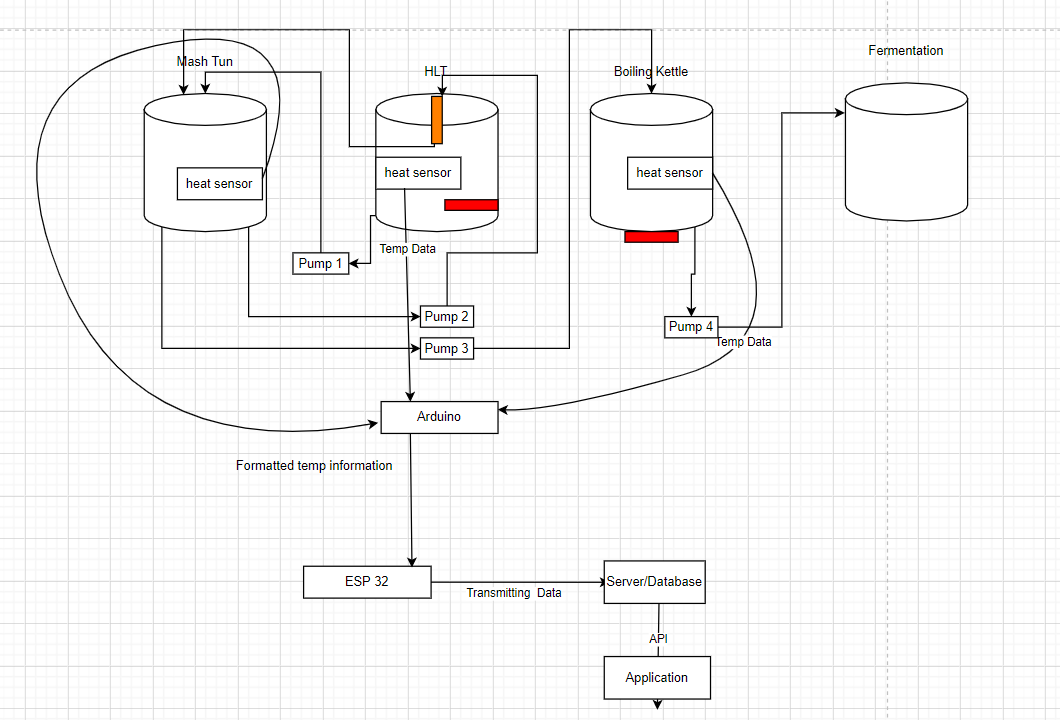
\includegraphics[scale=0.5]{images/sys_overview.PNG}
	\caption{System Overview}
\end{figure}
The Back Burner Brew will be a utilize four kettles as seen in figure 2 and the liquids will be transferred from each kettle through the use of pumps. The Back Burner Brew will have a user interface, both through a web application and a touch screen connected to a RaspberryPi. Through these interfaces, the brewer will be able to control the temperature of all the liquids inside of the Hot Liquor Tank (HLT) and the mash tun. Along with controlling the temperature, the user will be able to set when water from the HLT will be sent to the mash tun and when the mash tun will send the liquids through the HLT for heating. The liquds temperatures will be monitored through heat sensors and will be sending that data to the web application. The web application will display the current temperature of the liquids to the user and will have a kill switch in case the heating element does not control the temperature of the liquids as requested by the user.

The product will not control the temperature of the boiling kettle, rather the user will be able to control the power output of the heating element inside of the boiling kettle and will have to monitor the temperature and the amount of water loss through the boiling process. Because there will only be three pumps, the user must move connections manually between the pumps in order to have the liquid inside of the boiling kettle be transferred over to the cooler and fermentation kettle. The user must also add in the grains and hops into the different kettles depending on what stage of the brewing process they are in manually.
\subsection{External Inputs \& Outputs}
\begin{figure}[H]
	\centering
	\graphicspath{.\images}
	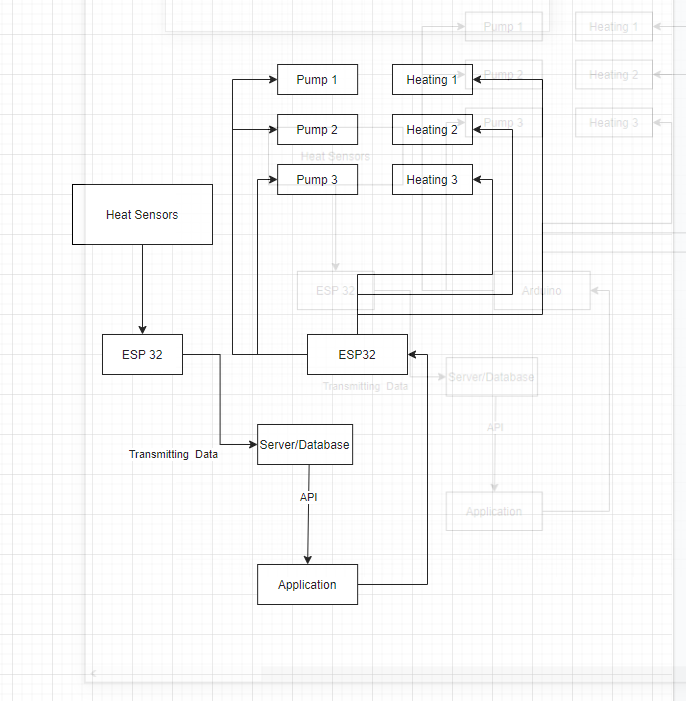
\includegraphics[scale=0.5]{images/data_flow.PNG}
	\caption{Data Flow and Control}
\end{figure}
The Back Burner Brew will utilize multiple ESP32's. The ESP32 will be used for reading the temperatures of the different kettles and the Arduino will be used to control the heating elements and the pumps as well.The ESP32 will read the temperatures of HLT and the mash tun and send them to web server. Once the data has been received by the server, the server will then display that data to the user on the web application. The server will also be able to tell the ESP32 which heating element must be turned on to maintain the desired temperature and which pump to turn on as well.

\subsection{Product Interfaces}
\begin{figure}[H]
	\centering
	\graphicspath{.\images}
	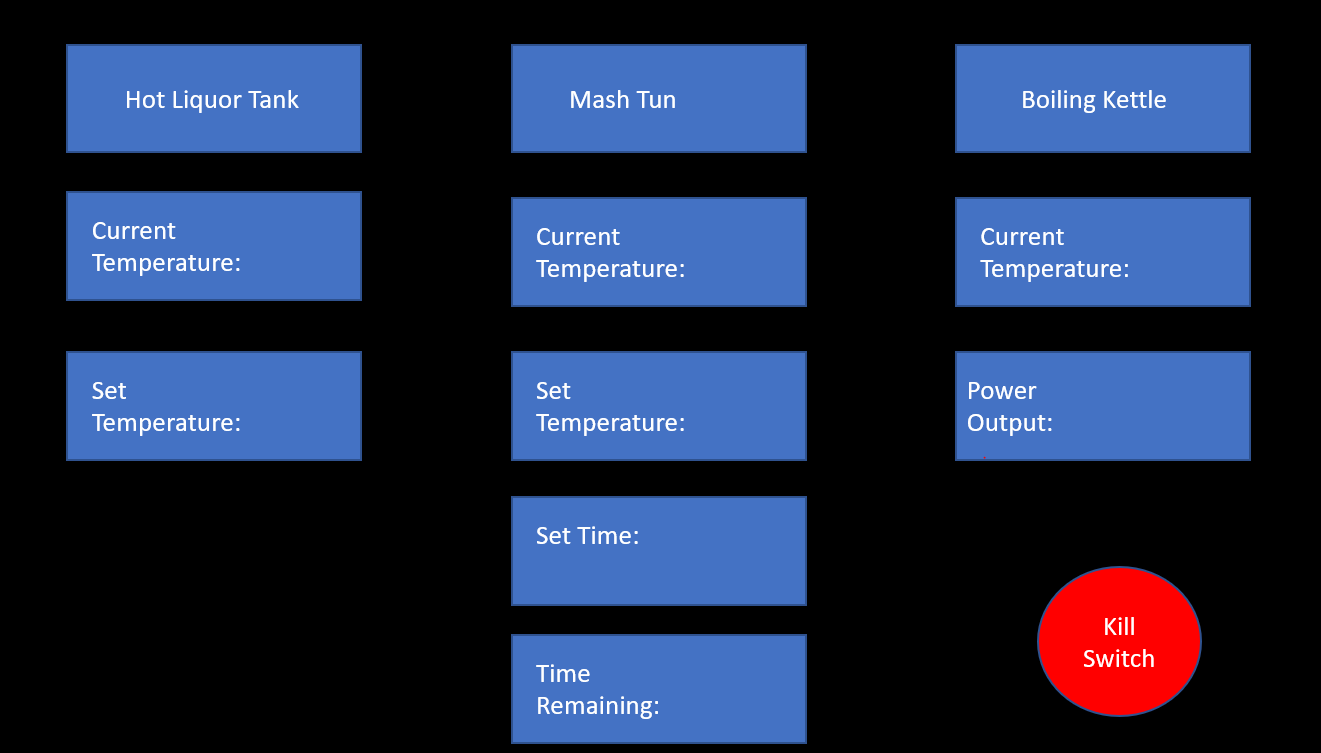
\includegraphics[scale=0.5]{images/web_page_template.PNG}
	\caption{Web Interface Template}
\end{figure}
The Back Burner Brew user interface template can be seen in the figure above. The web application will allow the user to set the temperature of both the HLT and the Mash Tun and will display the current temperatures as well. The mash tun will also allow for the user to enter the amount of time the mashing process will take, while also displaying the remaining time left on that process. The boiling kettle does not let the user control the temperature of the boiling kettle, rather, it lets the user control the power output of the boiling kettle and they must monitor the temperature of theboiling kettle themselves.
